\documentclass{article}
\usepackage{graphicx}

\begin{document}

\title{Context Switching Simulator V.0}
\date{\vspace{-5ex}}
\maketitle

\begin{enumerate}

\item Given Verilog design files, a Verilog testbench, and the name of the module to be swapped. 

\item Search for this module in the design. 

\item Traverse down the design starting from this module. 

\item Create a list containing all the state elements (registers and memories) in this module and all underlaying submodules recursively. 

\item Once a SAVE signal is asserted, the current state elements' values
will be saved in the list. 

\item Then, these elements are corrupted (by writing X or zeros), and simulation continues until a RESTORE signal is asserted. 

\item Once a RESTORE signal is asserted, the saved values are restored to
the state elements.

\end{enumerate}


\begin{center}
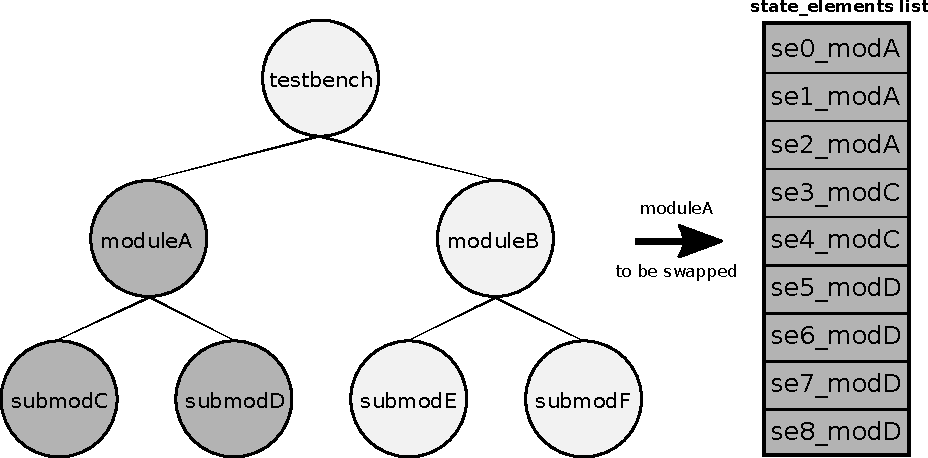
\includegraphics[width=14cm]{cssim_graph}
\end{center}

\end{document}
